\chapter{Deploy Frontend}
\label{Chapter5}
Sau khi tất cả service đã được chuẩn bị, ta tiến hành deploy \texttt{front-end} bằng \textbf{Vercel}.

\section{Deploy \texttt{front-end}}
Truy cập và tạo tài khoản \textbf{Vercel}. Sau đó, tạo một project mới và deploy từ GitHub repository của \texttt{front-end} đã được chuẩn bị.
Ta cũng có thể cấu hình thêm tên miền và domain riêng để deploy \textbf{Vercel}.

Tại cài đặt của project, truy cập vào mục Environment và cấu hình các biến môi trường sau:
\begin{enumerate}
    \item \texttt{VITE\_GATEWAY\_HOST}: Địa chỉ của tên miền API Gateway.
    \item \texttt{VITE\_STORAGE\_SERVICE\_HOST}: Địa chỉ truy cập xem storage của \texttt{AWS S3} đã cấu hình ở chương trước.
    \item \texttt{VITE\_UPLOAD\_API\_ENDPOINT}: Địa chỉ API Gateway dùng để upload avatar người dùng lên \texttt{AWS S3} đã cấu hình ở chương trước.
    \item \texttt{VITE\_UPLOAD\_COMPANY\_API\_ENDPOINT}: Địa chỉ API Gateway dùng để upload tài nguyên doanh nghiệp lên \texttt{AWS S3} đã cấu hình ở chương trước.
\end{enumerate}

\section{Kết quả}
Sau khi đã cài đặt thành công, ta có thể truy cập vào trang web của mình thông qua domain đã được cấu hình.

Ta cũng có thể nhìn thấy kết quả deploy tại trang quản lý của Vercel (Xem Hình ~\ref{fig:vercel}.

\begin{figure}
    \centering
    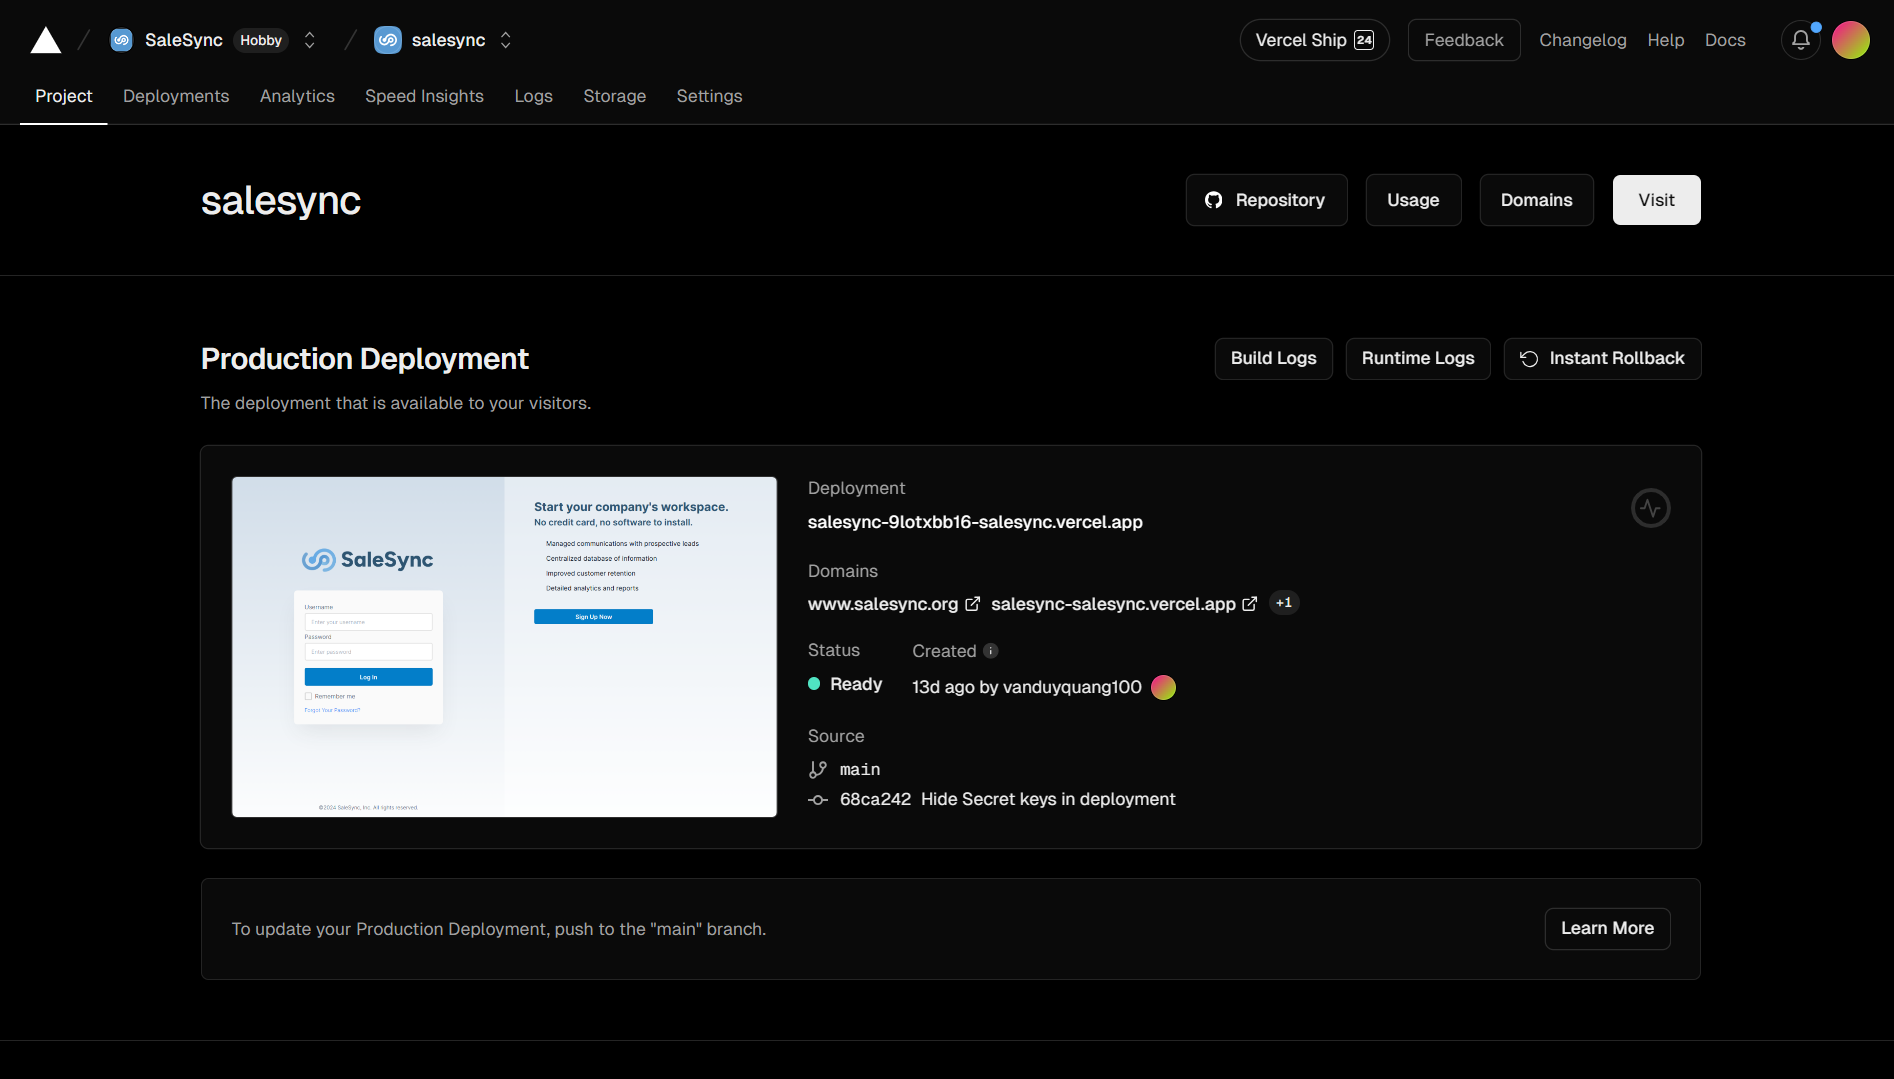
\includegraphics[width=1\linewidth]{vercel.png}
    \caption{Màn hình chính của Vercel}
    \label{fig:vercel}
\end{figure}

